\documentclass[
    a4paper,
    oneside,
    10pt
]{article}

\usepackage{lmodern}
\usepackage[utf8]{inputenc}
\usepackage[T1]{fontenc}
\usepackage[english, italian]{babel}

\usepackage[
	bindingoffset = 0.2in,
	left = 0.5in,
	right = 0.5in,
	top = 0.5in,
	bottom = 0.5in,
	footskip = 0.25in
]{geometry}
\usepackage{courier}

\usepackage{calc}
\usepackage{fontawesome5}
\usepackage{makecell}
\usepackage{longtable}
\usepackage{tikz}
\usepackage{xcolor}

\usepackage{graphicx}
\graphicspath{ {./db/} }

\newenvironment{timeline}{%
%	\renewcommand{\arraystretch}{1.2}%
%	\def\arraystretch{1.5}%
	\begin{longtable}{ c | c }%
}{%
	\end{longtable}%
}
\newcommand{\tldate}[1]{%
	\begin{minipage}[t]{2cm}%
		\begin{flushright}%
			\vspace{10pt}#1%
		\end{flushright}%
	\end{minipage}%
}
\newcommand{\tlcontent}[1]{%
	\begin{minipage}[t]{\textwidth-2cm}%
		\vspace{10pt}#1%
	\end{minipage}%
}

\begin{document}

    %==================== HEADER ====================%
    \begin{tabular}{ @{} c m{12cm} @{} }
		\begin{tikzpicture}[baseline=(ola.center),inner sep=0pt]
			\clip (0,0)  circle (2cm) node (ola) {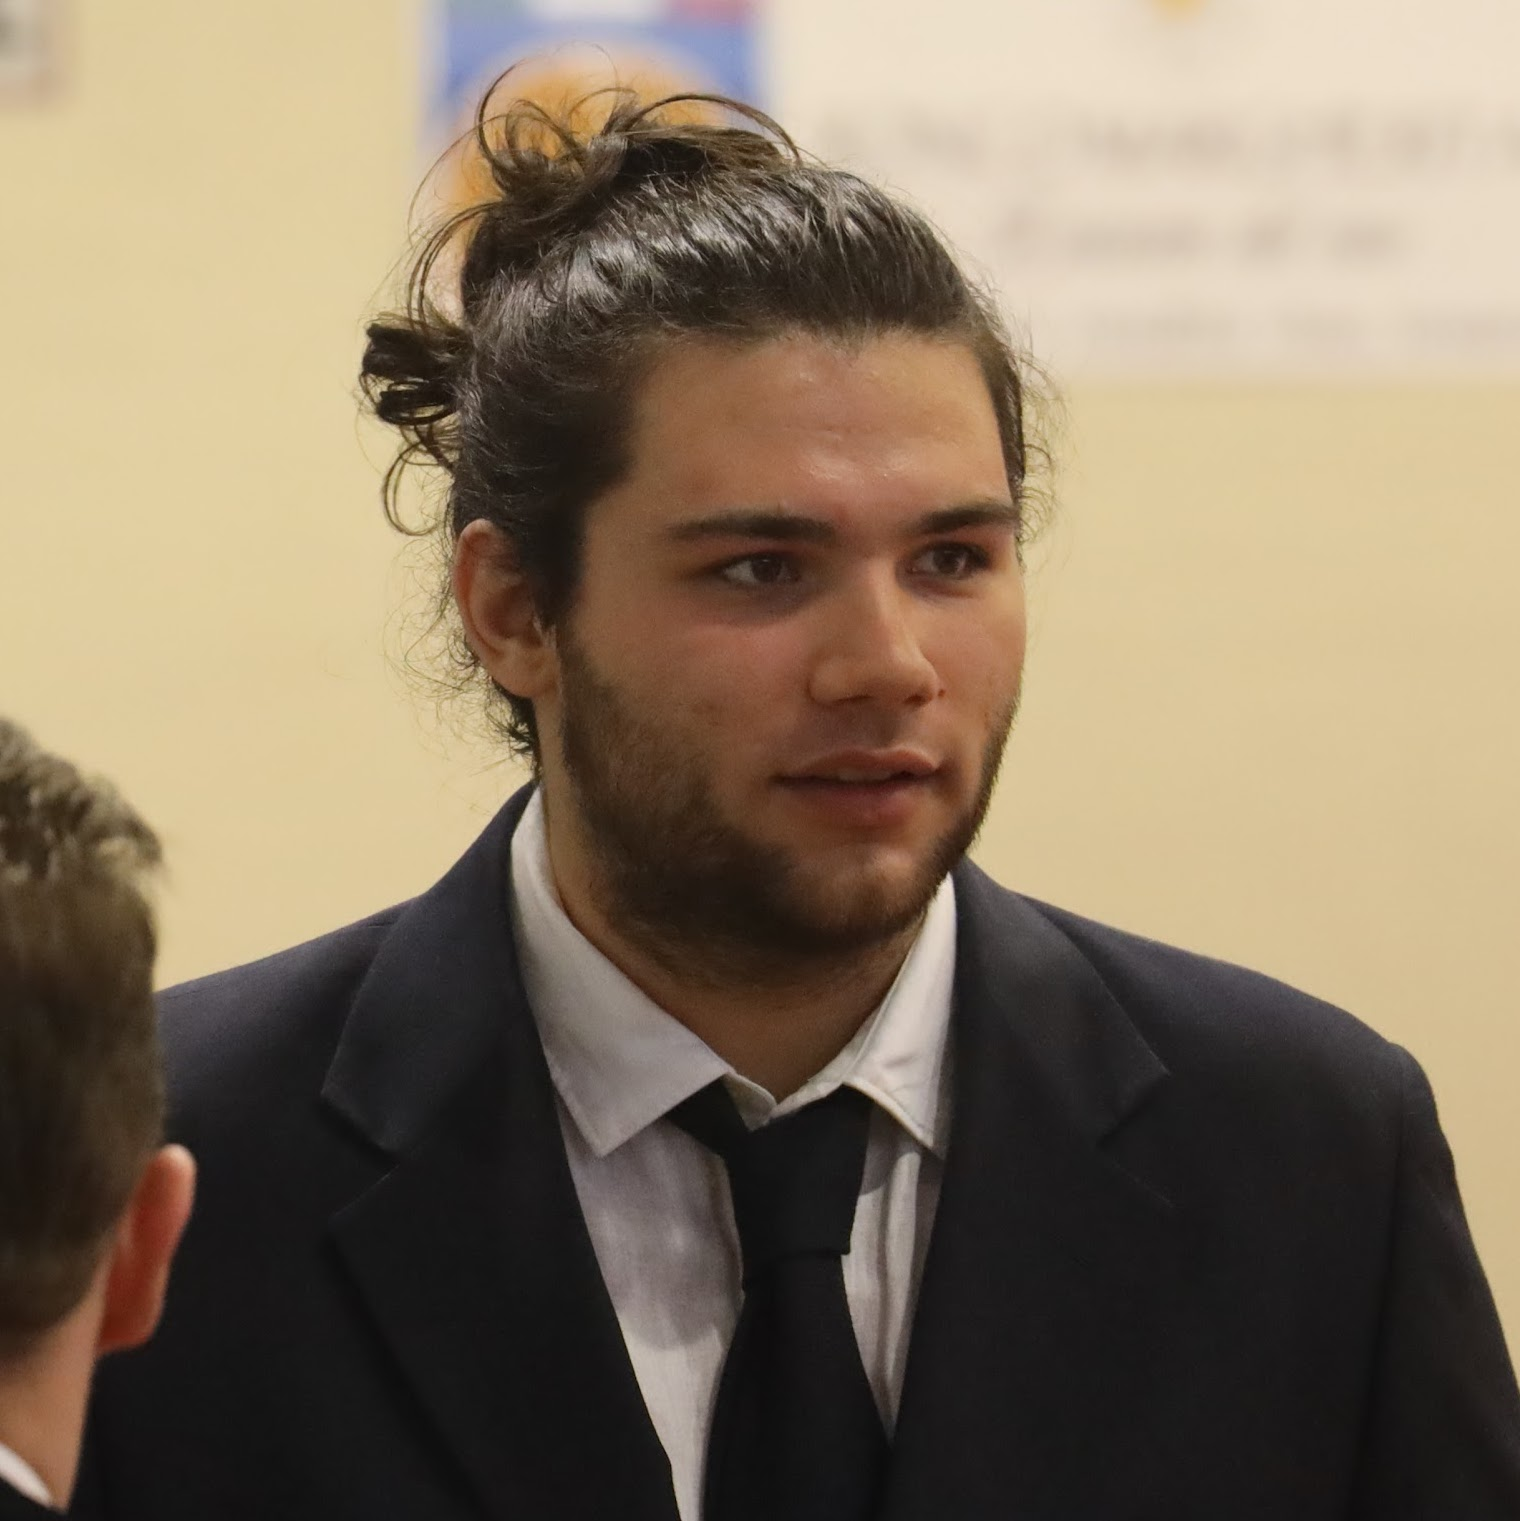
\includegraphics[height=4cm]{profile.jpg}};
		\end{tikzpicture} & \shortstack[l]{
			{\fontsize{25}{30}\selectfont\textbf{Urbani Ludovico}} \vspace{.3cm} \\
            {\fontsize{15}{20}\selectfont\textbf{Developer}}
		}
	\end{tabular} \\
	\begin{center}
		\begin{tabular}{ m{15cm} }
			\vspace{1cm} \\
			\hline
		\end{tabular}
	\end{center}
	\vspace{1cm}

    %==================== PROFILE ====================%

    \section{About}
	\begin{center}
		\renewcommand{\arraystretch}{1.25}
		\begin{tabular}{ r@{\hspace{.5cm}} | @{\hspace{.5cm}}l }
            Born & 2 June 2003 \\
			Fiscal Code & RBNLVC03H02L424F \\
			Living & Trieste (IT)
		\end{tabular}
	\end{center}

    \subsection{Contacts}
	\begin{center}
		\renewcommand{\arraystretch}{1.25}
		\begin{tabular}{ r@{\hspace{.5cm}} @{\hspace{.5cm}}l }
            \faAt & lu.urbani@outlook.com \\
			\faPhone & (+39) 331-2603770 \quad\faWhatsapp\;\faTelegram
		\end{tabular}
	\end{center}
	
    %==================== EDUCATION ====================%
    
    \section{Education}
    
    \begin{timeline}
    		\input{|python3 api/education.py}
    \end{timeline}

\end{document}